\documentclass[14pt]{extbook}
\usepackage{multicol, enumerate, enumitem, hyperref, color, soul, setspace, parskip, fancyhdr} %General Packages
\usepackage{amssymb, amsthm, amsmath, latexsym, units, mathtools} %Math Packages
\everymath{\displaystyle} %All math in Display Style
% Packages with additional options
\usepackage[headsep=0.5cm,headheight=12pt, left=1 in,right= 1 in,top= 1 in,bottom= 1 in]{geometry}
\usepackage[usenames,dvipsnames]{xcolor}
\usepackage{dashrule}  % Package to use the command below to create lines between items
\newcommand{\litem}[1]{\item#1\hspace*{-1cm}\rule{\textwidth}{0.4pt}}
\pagestyle{fancy}
\lhead{Progress Quiz 7}
\chead{}
\rhead{Version C}
\lfoot{4173-5738}
\cfoot{}
\rfoot{Spring 2021}
\begin{document}

\begin{enumerate}
\litem{
Construct the lowest-degree polynomial given the zeros below. Then, choose the intervals that contain the coefficients of the polynomial in the form $ax^3+bx^2+cx+d$.\[ \frac{2}{3}, \frac{1}{2}, \text{ and } \frac{-7}{2} \]\begin{enumerate}[label=\Alph*.]
\item \( a \in [11, 24], b \in [26, 35], c \in [-50, -44], \text{ and } d \in [14, 21] \)
\item \( a \in [11, 24], b \in [-29, -26], c \in [-50, -44], \text{ and } d \in [-16, -12] \)
\item \( a \in [11, 24], b \in [39, 45], c \in [3, 4], \text{ and } d \in [-16, -12] \)
\item \( a \in [11, 24], b \in [26, 35], c \in [-50, -44], \text{ and } d \in [-16, -12] \)
\item \( a \in [11, 24], b \in [50, 60], c \in [53, 61], \text{ and } d \in [14, 21] \)

\end{enumerate} }
\litem{
Which of the following equations \textit{could} be of the graph presented below?
\begin{center}
    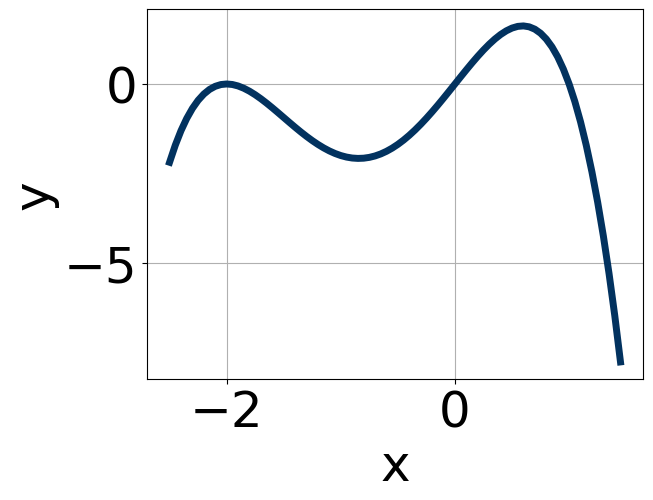
\includegraphics[width=0.5\textwidth]{../Figures/polyGraphToFunctionC.png}
\end{center}
\begin{enumerate}[label=\Alph*.]
\item \( 9x^{8} (x + 2)^{4} (x - 1)^{9} \)
\item \( -2x^{5} (x + 2)^{8} (x - 1)^{4} \)
\item \( 13x^{11} (x + 2)^{10} (x - 1)^{7} \)
\item \( -3x^{7} (x + 2)^{8} (x - 1)^{11} \)
\item \( -9x^{5} (x + 2)^{9} (x - 1)^{8} \)

\end{enumerate} }
\litem{
Describe the zero behavior of the zero $x = 5$ of the polynomial below.\[ f(x) = 8(x + 2)^{8}(x - 2)^{7}(x + 5)^{10}(x - 5)^{5} \]\begin{enumerate}[label=\Alph*.]
\begin{multicols}{2}\item 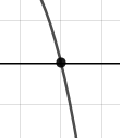
\includegraphics[width = 0.3\textwidth]{../Figures/polyZeroBehaviorAC.png}\item 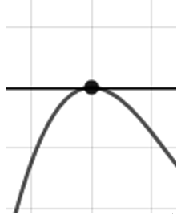
\includegraphics[width = 0.3\textwidth]{../Figures/polyZeroBehaviorBC.png}\item 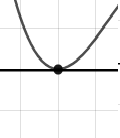
\includegraphics[width = 0.3\textwidth]{../Figures/polyZeroBehaviorCC.png}\item 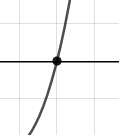
\includegraphics[width = 0.3\textwidth]{../Figures/polyZeroBehaviorDC.png}\end{multicols}\item None of the above.
\end{enumerate} }
\litem{
Construct the lowest-degree polynomial given the zeros below. Then, choose the intervals that contain the coefficients of the polynomial in the form $x^3+bx^2+cx+d$.\[ -4 - 3 i \text{ and } 2 \]\begin{enumerate}[label=\Alph*.]
\item \( b \in [-1, 4], c \in [-0.36, 1.69], \text{ and } d \in [-6.6, -3.6] \)
\item \( b \in [5, 9], c \in [8.74, 10.07], \text{ and } d \in [-50.9, -49.8] \)
\item \( b \in [-1, 4], c \in [1.92, 2.59], \text{ and } d \in [-10.8, -6.9] \)
\item \( b \in [-6, 0], c \in [8.74, 10.07], \text{ and } d \in [49.5, 51.7] \)
\item \( \text{None of the above.} \)

\end{enumerate} }
\litem{
Construct the lowest-degree polynomial given the zeros below. Then, choose the intervals that contain the coefficients of the polynomial in the form $ax^3+bx^2+cx+d$.\[ \frac{-7}{5}, \frac{1}{3}, \text{ and } \frac{1}{5} \]\begin{enumerate}[label=\Alph*.]
\item \( a \in [75, 82], b \in [-95, -92], c \in [-21, -16], \text{ and } d \in [1, 10] \)
\item \( a \in [75, 82], b \in [61, 66], c \in [-52, -46], \text{ and } d \in [1, 10] \)
\item \( a \in [75, 82], b \in [61, 66], c \in [-52, -46], \text{ and } d \in [-14, -6] \)
\item \( a \in [75, 82], b \in [-68, -60], c \in [-52, -46], \text{ and } d \in [-14, -6] \)
\item \( a \in [75, 82], b \in [-148, -139], c \in [57, 65], \text{ and } d \in [-14, -6] \)

\end{enumerate} }
\litem{
Describe the zero behavior of the zero $x = 3$ of the polynomial below.\[ f(x) = -2(x + 3)^{5}(x - 3)^{10}(x - 6)^{4}(x + 6)^{5} \]\begin{enumerate}[label=\Alph*.]
\begin{multicols}{2}\item 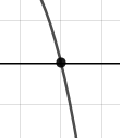
\includegraphics[width = 0.3\textwidth]{../Figures/polyZeroBehaviorCopyAC.png}\item 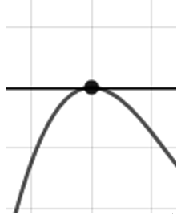
\includegraphics[width = 0.3\textwidth]{../Figures/polyZeroBehaviorCopyBC.png}\item 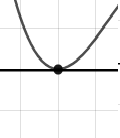
\includegraphics[width = 0.3\textwidth]{../Figures/polyZeroBehaviorCopyCC.png}\item 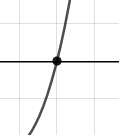
\includegraphics[width = 0.3\textwidth]{../Figures/polyZeroBehaviorCopyDC.png}\end{multicols}\item None of the above.
\end{enumerate} }
\litem{
Describe the end behavior of the polynomial below.\[ f(x) = 9(x - 7)^{3}(x + 7)^{8}(x + 8)^{3}(x - 8)^{4} \]\begin{enumerate}[label=\Alph*.]
\begin{multicols}{2}\item 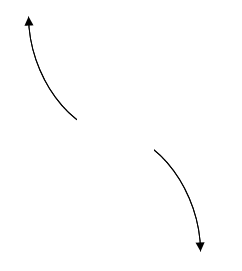
\includegraphics[width = 0.3\textwidth]{../Figures/polyEndBehaviorCopyAC.png}\item 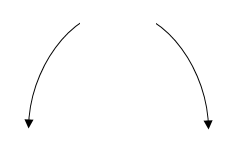
\includegraphics[width = 0.3\textwidth]{../Figures/polyEndBehaviorCopyBC.png}\item 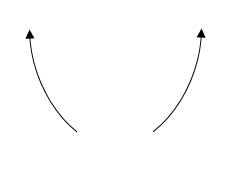
\includegraphics[width = 0.3\textwidth]{../Figures/polyEndBehaviorCopyCC.png}\item 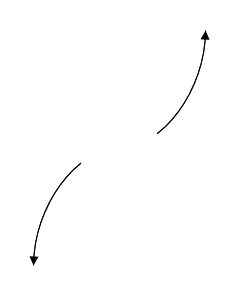
\includegraphics[width = 0.3\textwidth]{../Figures/polyEndBehaviorCopyDC.png}\end{multicols}\item None of the above.
\end{enumerate} }
\litem{
Describe the end behavior of the polynomial below.\[ f(x) = 4(x - 3)^{3}(x + 3)^{4}(x - 5)^{5}(x + 5)^{7} \]\begin{enumerate}[label=\Alph*.]
\begin{multicols}{2}\item 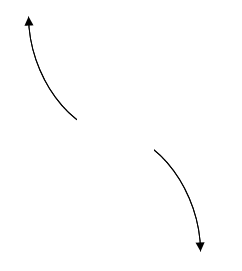
\includegraphics[width = 0.3\textwidth]{../Figures/polyEndBehaviorAC.png}\item 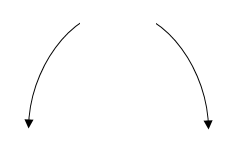
\includegraphics[width = 0.3\textwidth]{../Figures/polyEndBehaviorBC.png}\item 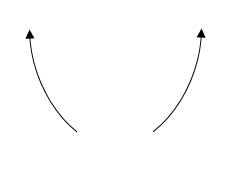
\includegraphics[width = 0.3\textwidth]{../Figures/polyEndBehaviorCC.png}\item 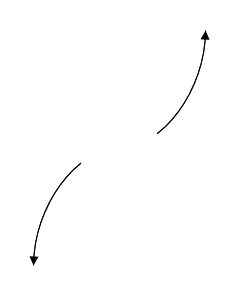
\includegraphics[width = 0.3\textwidth]{../Figures/polyEndBehaviorDC.png}\end{multicols}\item None of the above.
\end{enumerate} }
\litem{
Which of the following equations \textit{could} be of the graph presented below?
\begin{center}
    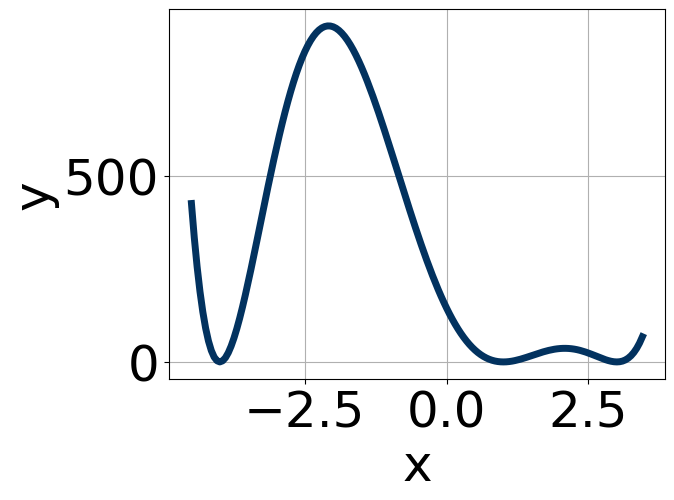
\includegraphics[width=0.5\textwidth]{../Figures/polyGraphToFunctionCopyC.png}
\end{center}
\begin{enumerate}[label=\Alph*.]
\item \( -20(x + 4)^{10} (x - 1)^{4} (x - 3)^{10} \)
\item \( 11(x + 4)^{4} (x - 1)^{5} (x - 3)^{11} \)
\item \( 5(x + 4)^{6} (x - 1)^{4} (x - 3)^{4} \)
\item \( 14(x + 4)^{6} (x - 1)^{10} (x - 3)^{7} \)
\item \( -8(x + 4)^{10} (x - 1)^{10} (x - 3)^{7} \)

\end{enumerate} }
\litem{
Construct the lowest-degree polynomial given the zeros below. Then, choose the intervals that contain the coefficients of the polynomial in the form $x^3+bx^2+cx+d$.\[ -4 + 2 i \text{ and } 4 \]\begin{enumerate}[label=\Alph*.]
\item \( b \in [2.8, 4.2], c \in [-12, -8], \text{ and } d \in [-83, -75] \)
\item \( b \in [0.1, 2.1], c \in [0, 3], \text{ and } d \in [-19, -12] \)
\item \( b \in [-6.4, -3.6], c \in [-12, -8], \text{ and } d \in [79, 82] \)
\item \( b \in [0.1, 2.1], c \in [-10, -2], \text{ and } d \in [7, 12] \)
\item \( \text{None of the above.} \)

\end{enumerate} }
\end{enumerate}

\end{document}